\documentclass[conference]{IEEEtran}
\usepackage{graphicx}
\usepackage{booktabs}
\usepackage{amsmath}
\usepackage{url}
\usepackage{xcolor}
\usepackage[hidelinks]{hyperref}

% Every \TBD must be filled from paper/results.md (full Session 5 runs), never from
% the 10-prompt trials. The trial value is kept in a comment next to each one for
% sanity-checking only. Delete this macro before submission: compile fails if any remain.
\newcommand{\TBD}[1][]{\textcolor{red}{[TBD#1]}}

\begin{document}

\title{Fewer Bits Save Energy Only With the Right Kernels:\\Measuring Precision and Energy in LLM Inference on a Shared GPU Cluster}

% TODO: check the venue's review policy (anonymous or not) before filling in.
\author{\IEEEauthorblockN{Author One, Author Two, Author Three}
\IEEEauthorblockA{Sardar Patel Institute of Technology, Mumbai, India\\
\{author\}@spit.ac.in}}

\maketitle

\begin{abstract}
Weight quantization is widely assumed to cut the energy of large language model (LLM) inference. We measure per-token GPU energy with the on-board hardware counter of an NVIDIA RTX~6000~Ada, for two inference stacks, two model sizes and two batch sizes, on a shared academic cluster. With bitsandbytes in Hugging Face Transformers, the most common drop-in path, quantization does not save energy: for Llama-3.2-1B at batch size~1, NF4 4-bit costs the same as float16 (1.6--1.7\,J/token) and LLM.int8 8-bit costs 1.8$\times$ more, because both dequantize to 16-bit at every step. With vLLM's native low-precision kernels, it does: for Llama-3.1-8B-Instruct, FP8 uses \TBD\ % trial: -38%
and AWQ 4-bit \TBD\ % trial: -65%
less energy per token than float16, at batch size 1 and 8, and FP8 saves \TBD\ % trial: -38%
at 1B. The saving comes from higher throughput at near-constant power. It is not free: 8B accuracy on knowledge and commonsense tasks is unchanged, but grade-school maths drops by 7 (FP8) and 14 (AWQ) points. We also report a measurement pitfall: on the shared node, daytime float16 measurements were inflated up to 7.7$\times$ by a host-side slowdown that passed an end-of-run co-tenancy check, repeat-run agreement and an automated validator, and we give a monitoring protocol that catches it. Finally, we evaluate per-prompt routing between precision tiers and between model sizes \TBD[: one-sentence routing result].
\end{abstract}

\begin{IEEEkeywords}
LLM inference, energy measurement, quantization, FP8, AWQ, vLLM, bitsandbytes, measurement methodology, routing
\end{IEEEkeywords}

\section{Introduction}
Quantizing an LLM's weights to 8 or 4 bits shrinks its memory footprint by 2--4$\times$, and a matching energy saving is often assumed. Whether it materialises depends on how the low-precision arithmetic is executed. The most widely used drop-in path, bitsandbytes in Hugging Face Transformers, stores weights in fewer bits but dequantizes them to 16-bit before every matrix multiply, and prior benchmarking found that this can raise inference energy~\cite{poddar2025}. Serving engines such as vLLM~\cite{kwon2023vllm} instead run kernels that compute in FP8 on the tensor cores or dequantize inside the matrix-multiply tile.

We set out to build a router that sends each prompt to the cheapest precision tier able to answer it, and found that on bitsandbytes there was no cheaper tier. This paper measures when fewer bits do and do not save energy, on hardware a typical academic group has: one shared two-GPU node. Our contributions:
\begin{enumerate}
\item \textbf{The kernel decides (§\ref{sec:results}).} Under bitsandbytes, 4-bit breaks even with float16 and 8-bit costs 1.8$\times$ more. Under vLLM, FP8 and AWQ 4-bit save \TBD\ and \TBD\ energy per token at 8B, at batch size 1 and 8. Power stays roughly constant; the saving comes from throughput.
\item \textbf{The price is paid in reasoning (§\ref{sec:acc}).} At 8B, knowledge and commonsense accuracy are unchanged while GSM8k drops by 7 and 14 points.
\item \textbf{A measurement pitfall and a protocol (§\ref{sec:pitfall}).} The same float16 model on the same GPU measured between 1.6 and 13.0\,J/token depending on time of day, while the GPU sat idle. Three standard safeguards accepted the inflated values. Continuous host and GPU monitoring catches it.
\item \textbf{Routing, measured (§\ref{sec:routing}).} A fuzzy per-prompt precision router used 38--49\% more energy than static float16 under bitsandbytes. With vLLM tiers and a 1B/8B model pair, \TBD[: routing result].
\end{enumerate}

\section{Related Work}
\textbf{Energy of LLM inference.} Poddar et al.~\cite{poddar2025} find that bitsandbytes 8- and 4-bit quantization raises inference energy to almost 2$\times$ at equal batch size (A6000, software estimators), with savings only from the larger batches quantization permits. TokenPowerBench~\cite{niu2026tokenpower} measures joules per token from 1B to 405B parameters, and Vellaisamy et al.~\cite{vellaisamy2026} decompose Llama-3.2-1B request energy on H100/H200. We add a controlled comparison of quantization \emph{implementations} on one GPU with a hardware counter, and the effect of shared infrastructure on the measurement itself.
\textbf{Measurement and quantization.} Zeus~\cite{you2023zeus} and LLMCarbon~\cite{faiz2024llmcarbon} measure or model deep-learning energy and carbon. LLM.int8()~\cite{dettmers2022int8} and NF4~\cite{dettmers2023qlora} target memory; GPTQ~\cite{frantar2023gptq} and AWQ~\cite{lin2024awq} target memory and accuracy, and vLLM~\cite{kwon2023vllm} serves them with fused kernels.
\textbf{Routing.} RouteLLM~\cite{ong2024routellm} and FrugalGPT~\cite{chen2023frugalgpt} route or cascade between different models for cost. We evaluate routing both between precision tiers of one model and between model sizes, with measured energy as the cost.

\section{Methodology}
\label{sec:method}
\textbf{Hardware.} NVIDIA RTX~6000~Ada (48\,GB, driver 610.43.02) in a shared two-GPU SLURM node (dual AMD EPYC, 224 threads); jobs request one GPU and 8 cores.

\textbf{Workload.} 500 deduplicated prompts (200 easy, 150 medium, 150 hard) from TriviaQA, Alpaca, GSM8K and CodeAlpaca; greedy decoding, at most 128 new tokens, seed 42, 5 discarded warm-up generations, one configuration resident at a time.

\textbf{Energy.} Energy per generation call is the change in the GPU's cumulative on-board counter (NVML \texttt{nvmlDeviceGetTotalEnergyConsumption}, mJ resolution) across the call. It is GPU-board energy only. In batched calls, energy is attributed to prompts in proportion to their output tokens.

\textbf{Stack A: bitsandbytes.} Llama-3.2-1B~\cite{llama3} in Transformers: NF4 4-bit with double quantization and float16 compute; LLM.int8(); float16. Each tier carries a LoRA adapter (Section~\ref{sec:acc} shows they do not help). Batch size~1. Energy per call is bracketed by \texttt{torch.cuda.synchronize()}; J/token is the median over prompts with $\geq$16 generated tokens, since the counter often does not advance for 1--2-token generations.

\textbf{Stack B: vLLM.} vLLM~\cite{kwon2023vllm} 0.31.0 with CUDA graphs and float16 activations. Tiers: float16; FP8 (dynamic per-tensor scales, on the Ada GPU's native FP8 tensor cores); AWQ 4-bit~\cite{lin2024awq} (Marlin kernels, public \texttt{hugging-quants} checkpoint). These kernels never materialise 16-bit weight matrices: FP8 multiplies in FP8, and Marlin dequantizes inside the matrix-multiply tile. Models: Llama-3.2-1B (float16, FP8) and Llama-3.1-8B-Instruct (float16, FP8, AWQ 4-bit). Batch sizes 1 and 8 (static batches of consecutive prompts). Each configuration runs in its own process. J/token is total energy over total output tokens. Three runs on different days \TBD[: say which were night/day].

\textbf{Monitoring.} For Stack B, a thread samples every 2\,s for the whole run: GPU utilisation, power and SM clock; other processes on our GPU (excluding vLLM's own engine process tree); host load average; and the clock of our pinned CPU cores. A configuration is excluded if a co-tenant appears or its median GPU utilisation while busy falls below 50\%.

\textbf{Accuracy.} lm-eval-harness on tinyMMLU, tinyGSM8k and tinyHellaswag (100 items each, IRT-estimated)~\cite{polo2024tiny}; the Transformers backend for Stack A and the vLLM backend for Stack B. Routing uses a reference-match proxy on our prompts (numeric match, normalised substring match, or token-F1 $\geq$ 0.5).

\section{Energy per Token by Precision}
\label{sec:results}

\textbf{Stack A: quantization does not save energy.} Three clean runs (on different nights) give 1.66--1.71\,J/token for 4-bit, 3.06--3.12 for 8-bit and 1.59--1.73 for float16 (Table~\ref{tab:bnb}). The 4-bit vs.\ float16 difference changes sign across runs ($+$1.4\%, $-$1.4\%, $+$4.4\%), so they are equal. float16 draws the most power but is fastest; the quantized tiers draw less power but run 1.4$\times$ (4-bit) to 2.8$\times$ (8-bit) slower, and the extra time costs more than the lower power saves.

\begin{table}[t]
\caption{Stack A (bitsandbytes, Llama-3.2-1B, batch 1), clean runs 5--7. Medians over prompts with $\geq$16 tokens.}
\label{tab:bnb}
\centering\small
\begin{tabular}{lccc}
\toprule
Tier & tok/s & W & J/token \\
\midrule
float16 & 80.7--81.8 & 130--142 & 1.59--1.73 \\
8-bit LLM.int8 & \TBD & \TBD & 3.06--3.12 \\
4-bit NF4 & \TBD & \TBD & 1.66--1.71 \\
\bottomrule
\end{tabular}
% TODO: fill 4-/8-bit tok/s and W from paper/analysis/tier_medians.csv (runs 5-7).
\end{table}

\textbf{Stack B: quantization saves energy.} Table~\ref{tab:vllm} gives per-token energy for every vLLM configuration. \TBD[: 2--3 sentences once the full runs are in: savings vs float16 per model and batch size with 95\% paired bootstrap CIs, spread across runs.]
% Trial (10 prompts, not citable), J/token bs1/bs8: 1b_fp16 0.967/0.244, 1b_fp8 0.597/0.170,
% 8b_fp16 5.323/1.091, 8b_fp8 3.281/0.670, 8b_awq4 1.859/0.364.

\begin{table}[t]
\caption{Stack B (vLLM): energy per output token, throughput and power, median over \TBD\ runs. Saving is relative to the same model's float16 at the same batch size, with 95\% paired bootstrap CI.}
\label{tab:vllm}
\centering\small
\setlength{\tabcolsep}{3pt}
\begin{tabular}{llcccc}
\toprule
Model & Tier & bs & J/tok & tok/s & Saving \\
\midrule
1B & float16 & 1 & \TBD & \TBD & -- \\
1B & FP8 & 1 & \TBD & \TBD & \TBD \\
8B & float16 & 1 & \TBD & \TBD & -- \\
8B & FP8 & 1 & \TBD & \TBD & \TBD \\
8B & AWQ 4-bit & 1 & \TBD & \TBD & \TBD \\
\midrule
1B & float16 & 8 & \TBD & \TBD & -- \\
1B & FP8 & 8 & \TBD & \TBD & \TBD \\
8B & float16 & 8 & \TBD & \TBD & -- \\
8B & FP8 & 8 & \TBD & \TBD & \TBD \\
8B & AWQ 4-bit & 8 & \TBD & \TBD & \TBD \\
\bottomrule
\end{tabular}
\end{table}

\textbf{Why the stacks differ.} Energy is power $\times$ time. In both stacks the quantized tiers draw similar or lower power than float16; what differs is time. Decoding at small batch sizes is limited by reading the weights from memory once per token. vLLM's FP8 and Marlin kernels read 2$\times$ and 4$\times$ fewer weight bytes and compute on them directly, so they decode faster and finish sooner at nearly the same power. bitsandbytes reads fewer bytes too, but then spends extra kernels dequantizing them to float16, which costs more time than the smaller read saves. \TBD[: confirm with measured W and tok/s from Table~\ref{tab:vllm}; note whether the saving is larger at 8B than at 1B, as the bandwidth argument predicts.]

\textbf{Batch size.} \TBD[: batching cuts J/token for every tier (trial: about 4--5$\times$ from bs 1 to 8); say whether relative savings hold at bs 8.] vLLM's float16 is itself \TBD\ cheaper per token than bitsandbytes' float16 for the same 1B model, so the serving stack matters even before quantization.
% Trial: vLLM 1b_fp16 bs1 0.97 vs bnb 1.59-1.73 J/token.

\section{Accuracy}
\label{sec:acc}

\begin{table}[t]
\caption{Accuracy (tinyBenchmarks, 100 items per task). Stack A tiers without and with their LoRA adapter.}
\label{tab:acc}
\centering\small
\setlength{\tabcolsep}{4pt}
\begin{tabular}{llccc}
\toprule
 & Configuration & MMLU & HellaSwag & GSM8k \\
\midrule
\multirow{6}{*}{A} & 1B float16 & 0.433 & 0.636 & 0.062 \\
 & \quad + adapter & 0.400 & 0.623 & 0.061 \\
 & 1B 8-bit & 0.391 & 0.634 & 0.104 \\
 & \quad + adapter & 0.388 & 0.640 & 0.075 \\
 & 1B 4-bit & 0.393 & 0.573 & 0.063 \\
 & \quad + adapter & 0.368 & 0.594 & 0.041 \\
\midrule
\multirow{5}{*}{B} & 1B float16 & 0.433 & 0.629 & 0.092 \\
 & 1B FP8 & 0.380 & 0.624 & 0.084 \\
 & 8B float16 & 0.629 & 0.818 & 0.746 \\
 & 8B FP8 & 0.640 & 0.823 & 0.674 \\
 & 8B AWQ 4-bit & 0.663 & 0.802 & 0.605 \\
\bottomrule
\end{tabular}
\end{table}

Table~\ref{tab:acc}. At 8B, FP8 and AWQ 4-bit stay within 3 points of float16 on tinyMMLU and tinyHellaswag, in both directions, which is within the noise of 100-item tasks. On tinyGSM8k, which requires multi-step arithmetic, FP8 loses 7.2 points and AWQ 4-bit 14.1. At 1B, FP8 loses 5.3 points on tinyMMLU and under 1 point elsewhere; GSM8k is near the floor for a 1B base model. Stack A's LoRA adapters lower tinyMMLU at every tier and do not help elsewhere. Note that our 1B model is the base model and our 8B model is instruction-tuned, so 1B vs.\ 8B accuracy is not a pure size comparison.

\section{Measurement Pitfall on a Shared Cluster}
\label{sec:pitfall}
Repeated Stack~A measurements of the same code and GPU reproduced closely for 4- and 8-bit, but float16 ranged from 1.59 to 12.97\,J/token (Table~\ref{tab:pitfall}). Accuracy and every routing decision were identical across runs; only time and energy changed.

\begin{table}[t]
\caption{Stack A float16 across runs of identical code on the same GPU.}
\label{tab:pitfall}
\centering\small
\begin{tabular}{lccc}
\toprule
Run & tok/s & W & J/tok \\
\midrule
S1, 3 runs (day)$^\dagger$ & 10.5--11.8 & 85 & 7.2--7.8 \\
Run 4 (day) & 6.2 & 81 & 12.97 \\
Runs 5--7 (night) & 80.7--81.8 & 130--142 & 1.59--1.73 \\
\bottomrule
\multicolumn{4}{l}{\footnotesize $^\dagger$Session~1 ran without LoRA adapters.}
\end{tabular}
\end{table}

\begin{figure}[t]
\centering
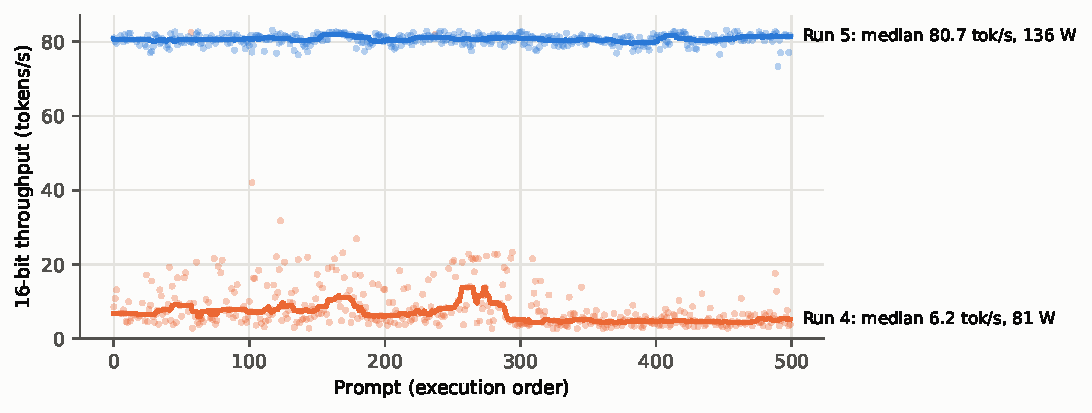
\includegraphics[width=\columnwidth]{figs/fig1_16bit_disruption.pdf}
\caption{Stack A float16 throughput per prompt in a disrupted (run 4) and a clean (run 5) run. Lines: rolling median over 25 prompts.}
\label{fig:disruption}
\end{figure}

\textbf{The signature.} Clean float16 runs are fast \emph{and} power-hungry: about 81\,tok/s at 130--142\,W, steady to within $\pm$1\,tok/s across the run (Fig.~\ref{fig:disruption}). Disrupted runs are slow \emph{and} low-power: 4--13\,tok/s at 81--85\,W, close to the GPU's mostly-idle draw. Since a waiting GPU still draws substantial power, energy per token rises roughly in proportion to the slowdown.

\textbf{Host-side, not GPU-side.} The GPU was not shared. A diagnostic timing plain float16 generation ran in daytime at 8.5\,tok/s on average with median GPU SM utilisation of 0\% and the process on-CPU 100\% of the time, and at night at 109.9\,tok/s: 13$\times$ faster on the same code and GPU. The GPU was waiting on a slowed CPU-side launch path. The node also runs CPU-only jobs that share the cores driving the GPU. \TBD[: Stack B day vs night comparison from the monitor logs: CPU clock, load, other processes; whether vLLM's CUDA graphs, which cut CPU launch work, made it less sensitive.]

\textbf{Why the safeguards missed it.} (1)~The co-tenancy snapshot was taken once, at the end of a run, and was empty for run~4. (2)~Session~1's three back-to-back runs agreed within 6.6\% and passed our pre-registered gate: agreement measured consistency, not cleanliness. (3)~The validator passed run~4, since its checks cannot see a uniform slowdown.

\textbf{Protocol.} Report throughput and mean power alongside J/token; check throughput stability across the run; sample GPU utilisation, co-tenants, host load and CPU clock continuously, not once; and exclude any configuration that departs from its clean baseline. Stack~B follows this protocol, and \TBD[: N of M configurations were flagged].

\section{Routing}
\label{sec:routing}
\textbf{Router.} A sensor computes five features per prompt (Flesch--Kincaid grade, approximate token length, character entropy, dependency-parse depth, a code/maths indicator), normalised to $[0,1]$. A Mamdani fuzzy controller (scikit-fuzzy; triangular memberships, seven rules, centroid defuzzification) maps them to a score in $[0,100]$, cut at 33/66 into a low, middle or high tier. It takes about 10\,ms per prompt on the CPU.

\textbf{Baselines.} Each static tier; \emph{random-matched}, with exactly the router's tier mix; \emph{learned}, a logistic regression on the same five features predicting whether the cheap option answers correctly, cross-fitted over 5 folds so no prompt is routed by a model that saw it; and an \emph{oracle} choosing the cheapest option that answers correctly. Greedy decoding lets every policy be evaluated from one prompt $\times$ configuration grid of measured energy and correctness.

\textbf{Stack A.} The fuzzy router used 65--76\,J/request more than static float16 in runs 5--7 (paired bootstrap; 38--49\% more energy) with no accuracy difference ($-$0.006, CI $-$0.034 to $+$0.020), and matched the oracle less often than a uniform random pick. With no tier cheaper than float16, routing had nothing to save.

\textbf{Stack B.} We evaluate two pools: precision tiers of the 8B model (AWQ 4-bit, FP8, float16), and the 1B and 8B models (1B float16 vs.\ 8B AWQ 4-bit). \TBD[: results table and 3--4 sentences from session5\_router\_replay.py: energy and proxy accuracy per policy vs.\ the best static option, with paired CIs; whether any policy beats static AWQ/FP8.]

\section{Threats to Validity}
One GPU model and one node. Two model families would strengthen generality; ours are both Llama. Static batches of 1 and 8, not continuous batching under load. GPU-board energy only, excluding CPU, DRAM and the router. The 1B model is a base model and the 8B is instruction-tuned. tinyBenchmarks tasks have 100 items each, so differences of a few points are within noise; the routing proxy metric is coarse. The host mechanism behind the Stack~A disruption is \TBD[: isolated / not isolated].

\section{Conclusion}
Whether fewer bits save energy in LLM inference depends on the kernel, not the bit-width. bitsandbytes 4-bit saves memory but not energy, and 8-bit costs 1.8$\times$ more than float16, because both compute in 16-bit after dequantizing. vLLM's FP8 and AWQ 4-bit kernels compute on the compressed weights and save \TBD\ and \TBD\ energy per token at 8B, at the cost of 7 and 14 points on grade-school maths. Measuring this on a shared cluster required monitoring the host, not just the GPU: a daytime slowdown inflated float16 energy up to 7.7$\times$ and passed every end-of-run safeguard. \TBD[: one sentence on routing.]

\bibliographystyle{IEEEtran}
\bibliography{refs}

\end{document}
